\documentclass[10pt]{beamer}

%\usepackage{lmodern}
%\usepackage[labelformat=empty,font=scriptsize,skip=0pt,justification=justified,singlelinecheck=false]{caption}

%\usepackage{paralist}
%\usepackage{amsmath}% http://ctan.org/pkg/amsmath
%\usepackage{amsfonts}% http://ctan.org/pkg/amsfonts

%\usepackage[font=scriptsize]{caption}

%\usepackage{hyperref}
\usepackage{amssymb,amsmath,amsfonts,eurosym,geometry,graphicx,caption,color,setspace,
comment,footmisc,caption,pdflscape,array}
\usepackage{booktabs}   % for nice tables
\usepackage{multirow}
%\usepackage[round]{natbib}
\setbeamertemplate{caption}[numbered]
\usepackage[export]{adjustbox}

\usepackage[skip=1pt]{caption}
%\usepackage[capposition=top]{floatrow}

%\usepackage[caption = false]{subfig}
%\usepackage{floatrow}
\usepackage[capposition=bottom]{floatrow}


%\usepackage{enumitem}%allow alphatebical ordering in enumerate
\usepackage{graphicx}
\usepackage{tabularx}
%\usepackage{threeparttable}
\usepackage{float}
\usepackage{mwe}
%\usepackage{subfig}
%\usepackage{polyglossia}
\usepackage{subcaption}
\setlength{\abovecaptionskip}{2pt}
%\usepackage[tight,TABTOPCAP]{subfigure}
\usepackage[round]{natbib}

\usepackage{multicol, latexsym, amsmath, amssymb}

\usepackage[normalem]{ulem}
\useunder{\uline}{\ul}{}
\usepackage{booktabs,caption}
\usepackage[flushleft]{threeparttable}

\usepackage{graphics}

\usepackage{longtable}

\usepackage{float}

\usepackage{amsbsy} %boldsymbol

%%in case of outdated TEX Live
\usepackage{lmodern}

\usepackage{appendixnumberbeamer}

%\graphicspath{{figures/}{../figures/}{D:/Presentations\figures/}}
\usepackage[normalem]{ulem}

\mode<presentation> {

% The Beamer class comes with a number of default slide themes
% which change the colors and layouts of slides. Below this is a list
% of all the themes, uncomment each in turn to see what they look like.

%\usetheme{default}
%\usetheme{AnnArbor}
%\usetheme{Antibes}
%\usetheme{Bergen}
%\usetheme{Berkeley}
%\usetheme{Berlin}
%\usetheme{Boadilla}
%\usetheme{CambridgeUS}
%\usetheme{Copenhagen}
%\usetheme{Darmstadt}
%\usetheme{Dresden}
%\usetheme{Frankfurt}
%\usetheme{Goettingen}
%\usetheme{Hannover}
%\usetheme{Ilmenau}
%\usetheme{JuanLesPins}
%\usetheme{Luebeck}
\usetheme{Madrid}
%\usetheme{Malmoe}
%\usetheme{Marburg}
%\usetheme{Montpellier}
%\usetheme{PaloAlto}
%\usetheme{Pittsburgh}
%\usetheme{Rochester}
%\usetheme{Singapore}
%\usetheme{Szeged}
%\usetheme{Warsaw}

% As well as themes, the Beamer class has a number of color themes
% for any slide theme. Uncomment each of these in turn to see how it
% changes the colors of your current slide theme.

%\usecolortheme{albatross}
%\usecolortheme{beaver}
%\usecolortheme{beetle}
%\usecolortheme{crane}
%\usecolortheme{dolphin}
%\usecolortheme{dove}
%\usecolortheme{fly}
%\usecolortheme{lily}
%\usecolortheme{orchid}
%\usecolortheme{rose}
%\usecolortheme{seagull}
%\usecolortheme{seahorse}
%\usecolortheme{whale}
%\usecolortheme{wolverine}

%\setbeamertemplate{footline} % To remove the footer line in all slides uncomment this line
%\setbeamertemplate{footline}[page number] % To replace the footer line in all slides with a simple slide count uncomment this line

%\setbeamertemplate{navigation symbols}{} % To remove the navigation symbols from the bottom of all slides uncomment this line
}
\usecolortheme{seahorse}

\usepackage{graphicx} % Allows including images
\usepackage{booktabs} % Allows the use of \toprule, \midrule and \bottomrule in tables

\usepackage{arydshln} %can use hdashline

\setbeamertemplate{footnote}{%
  \hangpara{2em}{1}%
  \makebox[2em][l]{\insertfootnotemark}\footnotesize\insertfootnotetext\par%
}
%----------------------------------------------------------------------------------------
%	TITLE PAGE
%----------------------------------------------------------------------------------------

\title[Task Specialization \& NF Wage Gap]{Price Discrimination} % The short title appears at the bottom of every slide, the full title is only on the title page

\author{Eduard Storm} % Your name
\institute[estorm@carleton.edu]
 % Your institution as it will appear on the bottom of every slide, may be shorthand to save space
{
	
	
	\medskip 
	
	Department of Economics \\  
	Carleton College \\ % Your institution for the title page
	\textit{estorm@carleton.edu} % Your email address
	
	\bigskip
	
	 Job Market Paper Presentation for: \\
		\smallskip
	EBS University of Business and Law
}


\date{January 13, 2021} % Date, can be changed to a custom date

\begin{document}

\begin{frame}
\titlepage % Print the title page as the first slide
\end{frame}

%----------------------------------------------------------------------------------------
%	PRESENTATION SLIDES
%----------------------------------------------------------------------------------------

\begin{frame} 
	\frametitle{Today's Game plan: Price Discrimination}
	
	
	\begin{enumerate}
		\item Motivation
		\item Perfect Price Discrimination (PPD)
		\item Extensions
	\end{enumerate}
	
	
\end{frame}
%------------------------------------------------
\begin{frame} 
	\frametitle{Motivational Example}
	
	
\begin{itemize}
	\item Tesla Models
	\item Colleges (especially in US) got better at price discrimination (815/1078) --> use Financial Literacy class as an example as it helped marginalized groups to enter college
	\item we know Higher Ed market has imperfect competition because Prices for college education differ (P at EBS different than in other universities)
\end{itemize}
	
	
\end{frame}
%------------------------------------------------

\begin{frame} 
	\frametitle{Poll}
	
\begin{center}
	\textbf{This is a poll}
\end{center}	

	
\begin{enumerate}%[label=(\Alph*)]
	\item 	1
	\item adsf
	\item adsf
	\item adsf
\end{enumerate}
	
\end{frame}
%------------------------------------------------

\begin{frame} 
	\frametitle{Perfect Price Discrimination (PPD)}
	
	Up until now, we only considered uniform pricing where each firm charges customers the same price
	
	\smallskip
	$\Longrightarrow$ Relax this assumption!\\
	\bigskip
	%%classification of PD goes back to Pigou (1920)
	\textbf{Key characteristics PPD}
	\begin{enumerate}
		\item Non-uniform pricing: Charge different customers different prices
			\begin{itemize}
				\item PPD commonly referred to as 1st degree PD
			\end{itemize}
		\item Consumers' preferences known
		\item Optimality requires: P = MB %bc demand curve is also the mb curve, it reveals customer's mb, thus also the max. price they're willing to pay - so in essense you set p right at the D curve
			\begin{itemize}
				\item Extensive margin: Make every possible sale
				\item Intensive margin: Charge each customer reservation price %will keep buying until MB=0, implying that reservation price equals mb where they are indifferent between buying or not
			\end{itemize}
		\item Conditions for PD
		\begin{itemize}
			\item Need market power (i.e. D downward-sloping)
			\item Prevent resales (e.g. Sony games), otherwise end up selling large Q at low P to resellers (otherwise they will undercut you)
			\item Target right customers with right P (--> transition to 2nd \& 3rd degree)
		\end{itemize}
	\end{enumerate}
	
\end{frame}
%------------------------------------------------

\begin{frame} 
	\frametitle{PPD: Graphical illustration}


 \begin{figure}[H]
	\centering
	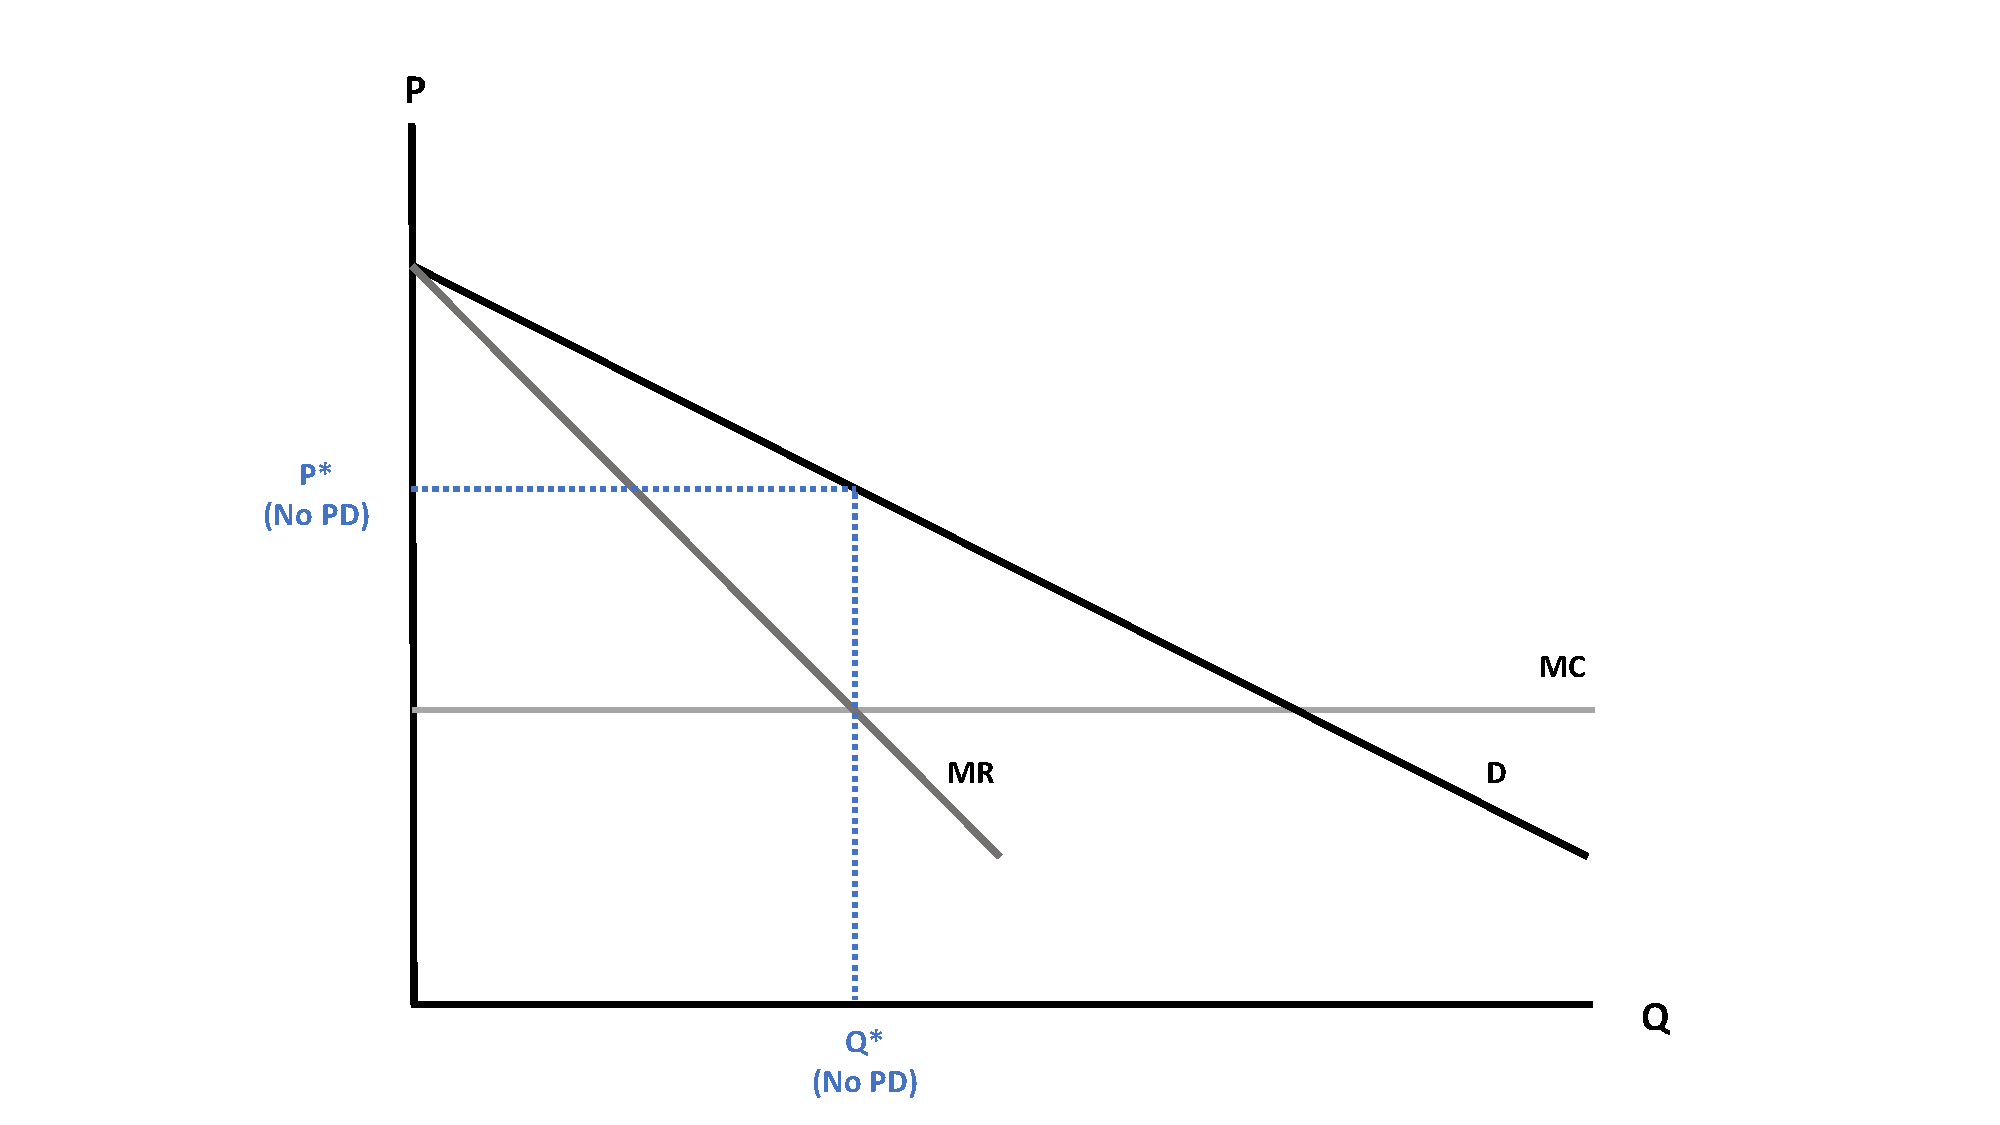
\includegraphics[width=0.9\linewidth]{no_pd}
	\caption{Monopolist: No Price Discrimination \\ 
\label{fig:nopd}}

\end{figure}

\begin{itemize}
	\item Optimality: MR = MC
\end{itemize}

%baseline:
%That’s the case we analyzed in Chapter 14, and hopefully you recall that a manager with market power first chooses their quantity at the point where marginal revenue equals marginal cost, then chooses their price by looking up to the blue demand curve. Consequently, with no price discrimination, everyone pays the same price, shown as the gray line in Figure 1.	
	
\end{frame}
%------------------------------------------------

\begin{frame} 
	\frametitle{PPD: Graphical illustration}
	
	
	\begin{figure}[H]
		\centering
		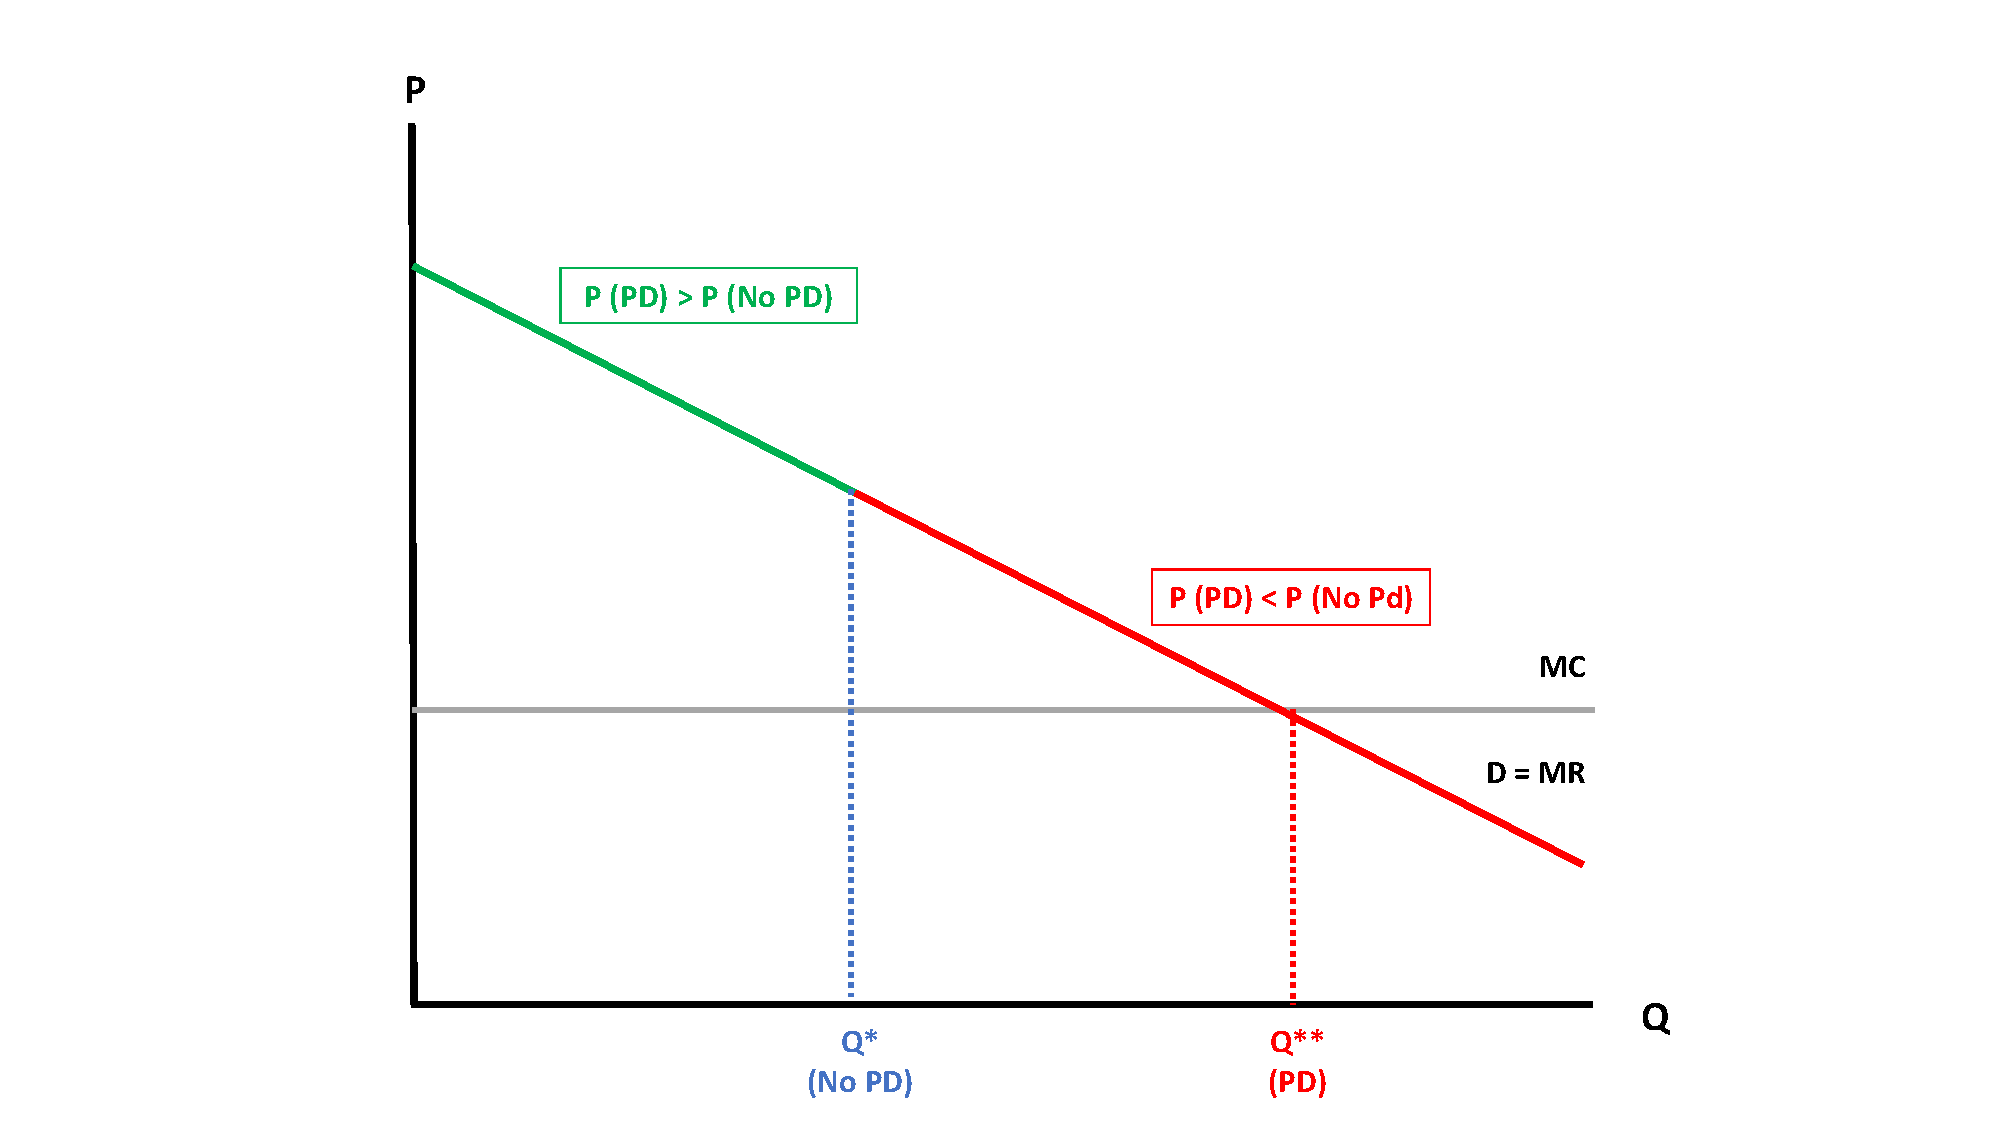
\includegraphics[width=0.9\linewidth]{pd}
		\caption{Monopolist: PPD \\ 
			\label{fig:ppd}}
		
	\end{figure}
	
	\begin{itemize}
		\item Optimality: P = MB
	\end{itemize}
	

\end{frame}
%------------------------------------------------

\begin{frame} 
	\frametitle{Poll}
	
	\begin{center}
		\textbf{What are the welfare implications of PPD?}
	\end{center}	
	
	\begin{enumerate}[(A)]
		\item Welfare-enhancing 
		\item Welfare-reducing 
		\item Welfare unchanged, surplus simply reduced
	\end{enumerate}

		
\end{frame}
%------------------------------------------------

\begin{frame} 
	\frametitle{PPD: Welfare}
	

	\begin{figure}[H]
		\centering
		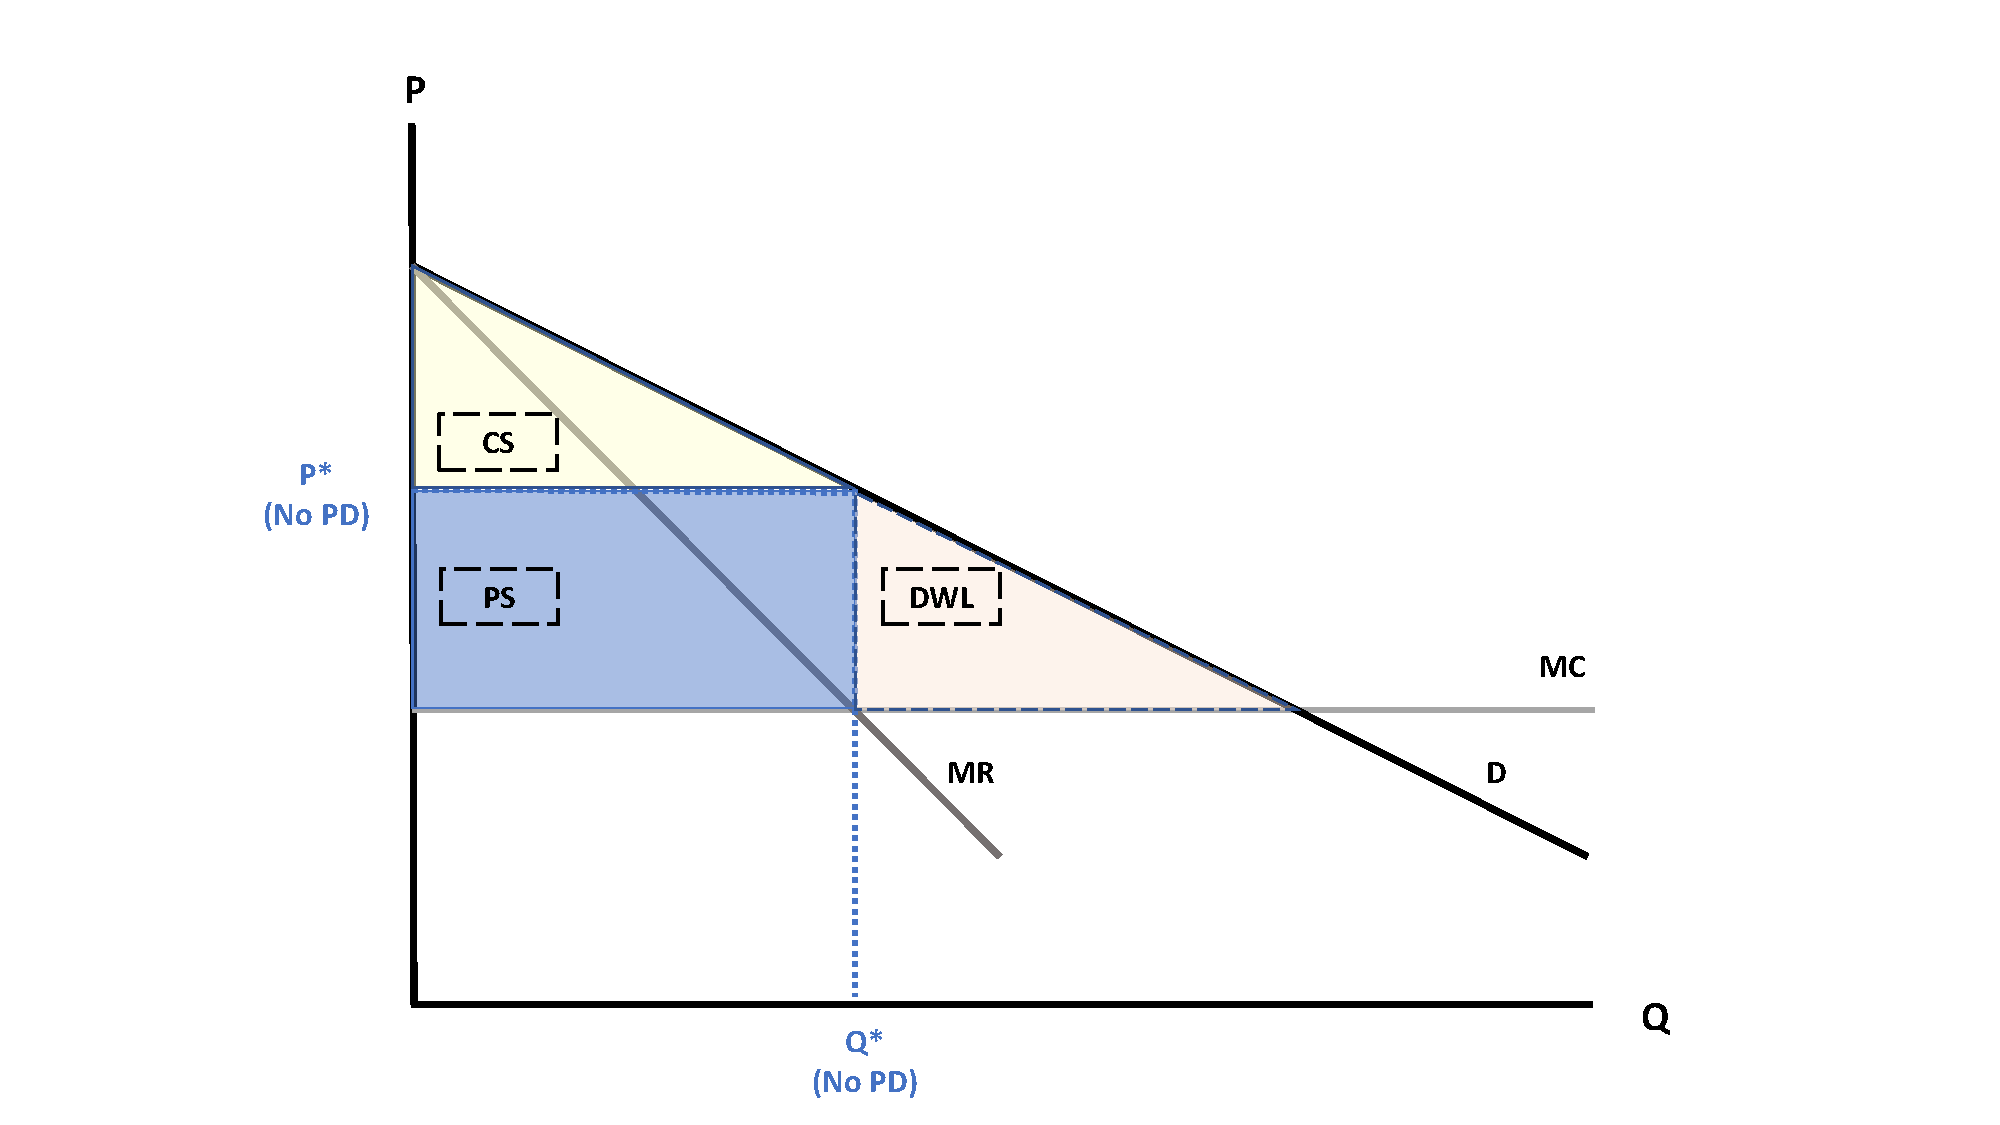
\includegraphics[width=0.8\linewidth]{no_pd_welf}
		\caption{Monopolist: PPD \\ 
			\label{fig:ppd}}
		
	\end{figure}
	
	\begin{itemize}
		\item Welfare: $\int_{0}^{Q*} (D - C) \,dQ = \underbrace{\int_{0}^{Q*} (D - P(Q)) \,dQ}_\text{CS} + \underbrace{\int_{0}^{Q*} (P(Q) - C)\,dQ }_\text{PS}$
	\end{itemize}
	
	
\end{frame}
%------------------------------------------------

\begin{frame} 
	\frametitle{PPD: Welfare}
	
	
	\begin{figure}[H]
		\centering
		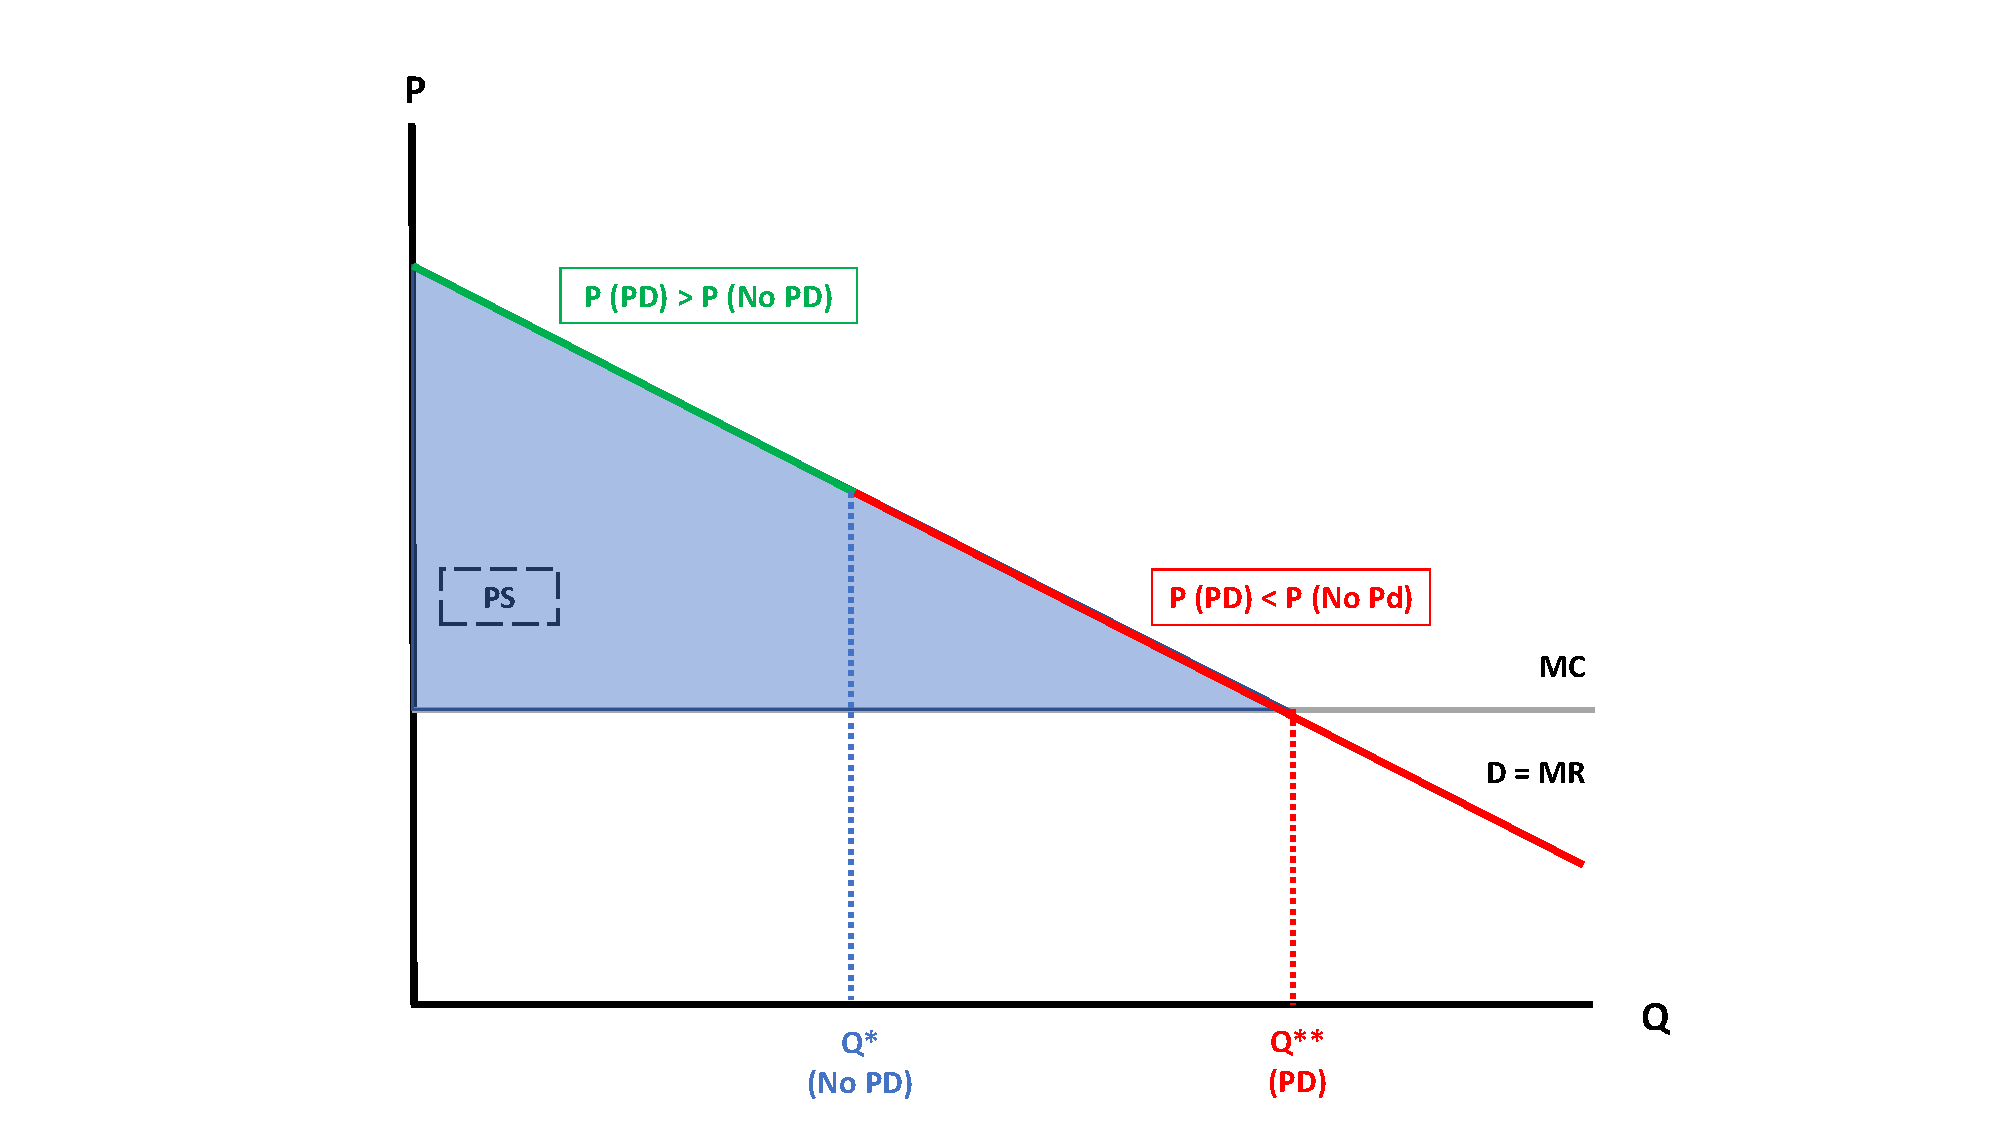
\includegraphics[width=0.8\linewidth]{pd_welf}
		\caption{Monopolist: PPD \\ 
			\label{fig:ppd}}
		
	\end{figure}
	
	\begin{itemize}
	\item Welfare: $\int_{0}^{Q**} (D - C) \,dQ = \underbrace{\int_{0}^{Q**} (P(Q) - C)\,dQ }_\text{PS}$
\end{itemize}
	
	
\end{frame}
%------------------------------------------------

\begin{frame} 
	\frametitle{Notes - Price Discrimination}
	
	\begin{itemize}
	\item \textbf{TO DO:} for preparation take a closer look at adjustments compared to more standard cases (also Ch. 14 in which firms exploit market power)
	\item check out basics on PC, Monopoly, Oligopoly	(e.g. why intuitively does monopolist not discrimiate and go beyond mr=mc (see figure 1)), \textbf{I think b/c then, w/o PD, would have to offer lower P to each customer and the price effect would lead to sub-optimal decision}

		
	\end{itemize}
	
%In the future, Sony hopes to do an even better job at preventing resale, and it is trying to shift movie and videogame distribution from sales of discs to online streaming, partly because these online streams can’t be copied or resold.	
	
\end{frame}
%------------------------------------------------

\begin{frame} 
	\frametitle{Notes - Extensions}
	
General Problem: Incomplete Information (don't typically know customer's reservation price) - that's why in reality we observe non-perfect discrimination (include somewhere that new technologies make that easier) 

	\begin{itemize}
		
		\item 2nd degree, non-linear pricing 
			\begin{itemize}
				\item hurdle method (rely on self-selection)
				\item quality differences (flying, car models)
				\item non-linear pricing
				\item Profit max. subject to (i) individual rationality constraints and (ii) incentive-compatibility constraints 
			\end{itemize}
		\item 3rd degree (group-specific, i.e. market segmentation, most common type)
		\begin{itemize}
			\item $MR_{1}=MR_{2}=MC$
			\item welfare: may improve due to higher output, yet, depends on degree of divergence between P \& MC
		\end{itemize}
	\end{itemize}
	
	%baseline:
	%That’s the case we analyzed in Chapter 14, and hopefully you recall that a manager with market power first chooses their quantity at the point where marginal revenue equals marginal cost, then chooses their price by looking up to the blue demand curve. Consequently, with no price discrimination, everyone pays the same price, shown as the gray line in Figure 1.	
	
\end{frame}
%------------------------------------------------


\end{document}